%
%   Chapter Introduction
%
%   author: Qing-Cheng Li r01922024 at csie dot ntu dot edu dot tw
%
\chapter{緒論}
\label{c:intro}

近年來,隨著網際網路的快速發展,網際網路中開始出現越來越多彙整人類知識的網站與資源,
如Wikipedia\footnote{http://www.wikipedia.org/},目前已經有超過280種語言,其中光是英語的條目就超過4,500,000條,
是透過來自世界各地的志願編輯者一字一句的貢獻建立而成的。

除了讓世界各地的人們可以在網際網路上共享知識之外,也讓計算機得以利用人類的知識,
輔助、改善、甚至自動化人工智慧、資料探勘與擷取、知識汲取、自動問答系統等任務,

為了達成此一目的,讓計算機可以看懂人類的知識,於是,
便出現了各式各樣透過擷取人工建立的知識資源,產生的結構化知識資料庫,並彼此相互鏈結。
如圖\ref{i:lod}所示,目前已有不少的結構化知識庫。
這些各式各樣的資源的最源頭,還是透過人類一字一句編輯產生的。% FIXME

\begin{figure}
\centering
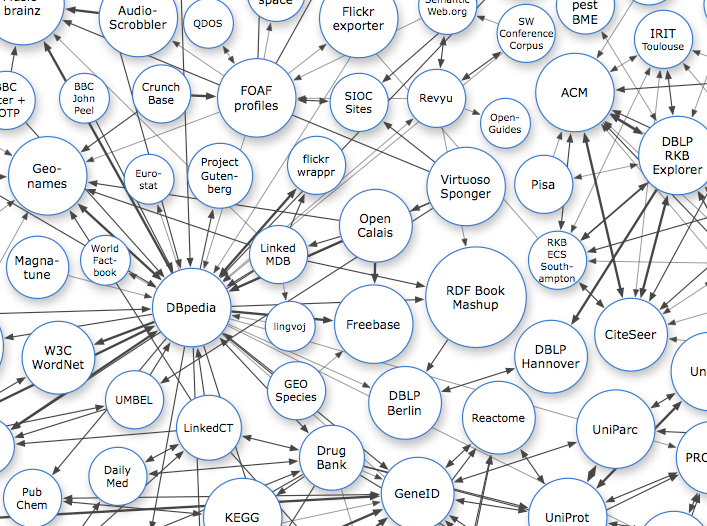
\includegraphics[width=0.5\textwidth]{images/01-lod-datasets}
\caption{各種結構化知識資料庫之間的鏈結}
\label{i:lod}
資料來源:linkeddata.org(2011)
\end{figure}

%
%   Background
%
\section{背景介紹}
在現今這個資訊社會,每當有新的事件發生時,例如某人的出生或死亡、某政治人物贏得了選舉、某地發生了天災等等,
這些資訊便會在網路上透過網路新聞、網誌、論壇、社群網站、微網誌等管道流傳。
新事件的發生代表了一些舊有的知識可能需要更新,例如修改某個人物的生死狀態、某個政治人物的勝選記錄等,
如有Wikipedia的志願編輯者注意到這些資訊之後,便會據此更新Wikipedia上關於某人或某球隊的條目。

如Wikipedia這種用來記錄實體(Entity)、實體的特性(Properties)、實體與實體間的關係(Relationships)的資料庫被稱為知識庫(Knowledge Base)。
以Wikipedia來說,Wikipedia以文章的形式儲存了人物、組織、公司、城市、事件等實體,
並在文章的文句中以超連結(Hyperlink)的形式描述實體與實體間的關係。
而文章中的資訊框(Infoboxes)則以半結構化的形式描述了實體的特性,如圖\ref{i:wiki}。

\begin{figure}
\centering
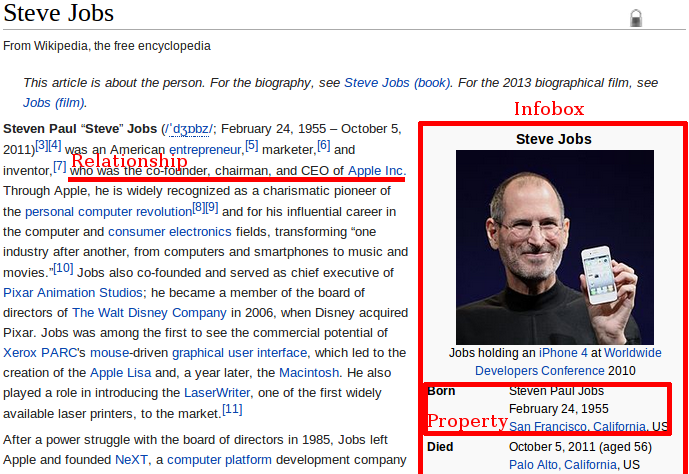
\includegraphics[width=0.65\textwidth]{images/01-wiki-as-kb}
\caption{Wikipedia中的文章}
\label{i:wiki}
\end{figure}

除了Wikipedia之外,還有其他DBpedia\cite{dbpedia-swj}、YAGO\cite{suchanek2007WWW}、Freebase\cite{freebase}等規模大小不一、不同應用的知識庫。
其中YAGO、DBpedia是透過自動化的方法擷取Wikipedia的內容,Freebase仰賴社群更新,這些知識庫都直接或間接仰賴人力更新。  %FIXME

%
%   Motivation
%
\section{研究動機}
% 知識庫不會憑空產生,多半是擷取人工編輯的成果或靠人工編輯,因此如何讓人工編輯的速度可以跟上知識產生的速度便成為一個重要的課題。
% TODO
% Keyword: 知識庫加速
知識庫的維護者,如Wikipedia的志願編輯者,人數比起知識庫中的實體實在是非常的少, % FIXME -> 這裡是翻自KBA
這意味著當舊有的知識產生變化時,或有新的知識出現時,這樣的變動或新增需要經過一段長時間後,編輯者才會更新知識庫。
% TODO - 補一下數據,大概多久才會被更新的數據
為了縮短新知識產生到更新知識庫的這段差距,自2012年起至今的每年NIST的TREC(TExt Retriveal Conference)都會舉辦KBA(Knowledge Base Acceleration)競賽,
提供一個有4973小時,每個小時包含100000篇文件的的內容串流(Content Stream),模擬現實世界之中不斷產生的新文章,包含了新聞、部落格、論壇等。
並給定了一組關注的實體,包含了人物、組織或建築,希望參賽者可以建立一個系統過濾內容串流中的資訊,
推薦編輯者哪些資訊可以幫助編輯者更新知識庫中關於這些目標實體的知識。
% TODO - 補一下 KBA 數據

% TODO
% We want to fill the Knowledge gap, do it fast

%TODO - Add KBA overview's image

%由於每天產生的資訊太多,與知識庫的更新落差太大,我們希望可以縮短這樣的差距,加速知識庫的更新。



%
%   Goal
%
\section{研究目標}
% Keyword: given a content stream, 回答有沒有某個特性這樣
% TODO

%
%   Structure
%
\section{論文架構}  % TODO FIXME
本論文共分成五個章節。
第一章是緒論,簡介本研究的背景、動機與目標。
第二章是文獻探討,列舉了一些相關的研究與資源。
第三章是研究方法,提出如何於內容串流中究偵測實體特性的方法與步驟。
第四章是實驗結果與分析,
第五章是結論與未來展望,

